\documentclass[handout]{beamer}

\usepackage[french]{babel}
\usepackage[utf8]{inputenc}
\usepackage{listings}

\usetheme{Warsaw}

\title{TP - Programmation Orientée Objet}
\author{Romain PELISSE}
\institute{
ESME Sudria \\ 
\\
\\

\includegraphics[scale=0.3]{../img/logo-cc.png}
}
\date{\today}

%\logo{}

\begin{document}
% Definition de l'affichage de l'ensemble des codes
	\definecolor{white}{rgb}{1,1,1}
	\definecolor{monbleu}{rgb}{0.03, 0.45, 0}
	\lstset{
		language=Java, 
		backgroundcolor=\color{white}, 
		basicstyle=\small, 
		commentstyle=\color{monbleu},
		keywordstyle=\color{blue}\bfseries\emph
	}

% end...
\frame{\titlepage}

\section[Agenda]{}
\frame{\tableofcontents[part=1]}
\part{1}
\section{Rappel}
\subsection{Notions de base}
\begin{frame}
	\frametitle{Notions de Base}
	La compréhension des notions suivantes est un \emph{prérequis} {\`a} la réalisation de ce tp :
	\begin{itemize}
		\item<1-> Classe et Objet
		\item<2-> Constructeurs et Destructeurs
		\item<3-> Visibilité des classes, méthodes et variables ( private, public, protected,...)
		\item<4-> Héritage et Polymorphisme Dynamique
		\item<5-> Surcharge de méthodes et d'opérateurs
	\end{itemize}
	\textit<6->{Si vous avez des doutes ou des questions sur ces notions, c'est le moment !}
\end{frame}


\section{Différences entre le Java et le C++}

\begin{frame}
	\frametitle{Différences conceptuelles}
	\begin{block}{C++}
		\begin{itemize}
% Le C++ est une ``surcouche'' au C. Il étend le langage C pour lui donner les capacités d'un langage Objet. 
% Le C++ est très puissant, mais aussi très complexe, il requiert une très bonne maîtrise du langage ( qui est le langage au monde possédant le plus de mot-clés !) mais aussi des connaissances poussées en termes de conception objet. 
% Ajouté à cela, il requiert de la part du développeur une bonne gestion de la mémoire.
			\item Simple \textit{surcouche objet} au C et non un ``pur`` langage Objet,
			\item Puissant mais \textbf{complexe}, utilise \textbf{beaucoup de mot-clés},	
			\item La \textbf{libération de la mémoire} est à la charge du développeur,
			\item Le langage est peu structurant dans l'organisation des fichiers.
		\end{itemize}
	\end{block}	
	\begin{block}{Java}
		\begin{itemize}
% Le Java est un langage ''très objet`` et non une simple surcouche à un langage procédural comme le C. 
% De plus, il limite volontairement le nombre de mots-clés. Le Java se veut avant tout simple et structurant.
% Dernier point,en Java, la libération de la mémoire se fait de manière automatique.
			\item Langage \textit{très orienté} objet,
			\item Syntaxe \textbf{simple} et structurante, \textbf{peu de mots-clés},
			\item Gestion automatique de la \textbf{libération mémoire},
			\item Une classe = un fichier (imposée par le compilateur).
		\end{itemize}
	\end{block}

% 	\begin{center}
% 		\textit{Attention, ceci ne signifie pas que Java est facile et que C++ est complexe mais
% 		seulement que les principes de bases régissant ces langages sont similaires mais reposent 
% 		sur des philosophies différentes.}
% 	\end{center}
\end{frame}


\subsection{Héritage en Java}
%^\subsection{Super classe Object}
\begin{frame}
	\begin{block}{La ``super'' classe 'Object'}
	Tout objet hérite de manière implicite de 'Object':
		\begin{itemize}
			\item 'String toString()' retourne l'objet sous forme de chaîne.
			\item 'boolean equals(Object other)' permet de comparer 2 objets.
			\item 'Class getClass()' qui permet de récupérer une instance de la classe de l'objet ( voir plus loin la partie sur la réflexion ).
%			\item ... et quelques autres qui dépassent le cadre du TP
		\end{itemize}
	\end{block}

	\begin{block}{Héritage implicite}
		\lstinputlisting[first=3,last=4]{../examples/org/esme/samples/ImplicitInheritance.java}
	\end{block}
% Exemple peu pertinent...	 	\lstinputlisting[first=2,last=13]{../examples/org/esme/samples/ImplicitInheritanceExample.java}
\end{frame}

%^\subsection{Abscence d'héritage multiple}

\begin{frame}
	\frametitle{Absence d'héritage multiple}
% 	Le Java, à l'inverse du C++, n'autorise pas l'héritage multiple. Ceci autant pour simplifier le code
% 	( les héritages multiples rendent le code plus complexe ) que parce que l'utilisation d'héritage
% 	multiple est généralement admise comme une mauvaise pratique. 
% 	Donc, en Java, tout objet hérite directement ou indirectement de Object ( voir plus loin ), mais en aucun cas de
% 	plusieurs classes. Pour obtenir un effet ``similaire'' à l'héritage multiple ( soit attribut à une
% 	classe plusieurs ``nature'' ), on utilise les interfaces ( voir plus loin ).

	\begin{block}{Pourquoi il n'y a pas d'héritage multiple ?}
		\begin{itemize}
			\item \textbf{Simplicité}, le code est moins complexe, la hiérarchie des classes est plus claire
			\item L'héritage multiple est reconnu comme une ``\textbf{bad practice}``
			\item Les \textbf{Interfaces} sont utilisées à la place 
		\end{itemize}
	\end{block}

\end{frame}

\subsection{Gestion de la mémoire}

\begin{frame}
	\frametitle{Gestion automatique de la mémoire}
% 	A l'inverse du code binaire généré par le C++, qui est interprétable par un processeur précis, la 
% 	compilation d'une classe Java (avec \textbf{javac}) aboutit à la génération d'un \textit{bytecode} qui
% 	ne correspond pas à une architecture physique ( PowerPPC, Intel x86, ...) mais à un code binaire
% 	interprétable par la machine virtuelle Java (\textit{Java Virtual Machine - JVM}).
% 	La machine Java est un programme, compilé pour une achitecture précise lui, qui se chargera
% 	d'exécuter le code associé.
	\begin{block}{Le \textit{bytecode}}
		\begin{itemize}
			\item Compilation génère du \textit{bytecode}, soit du code binaire.
			\item Le \textit{bytecode} est interprétable par la machine Java et non par le processeur physique ( PowerPPC, Intel, Vax,... )
			\item Java se charge de l'interprétation du \textit{bytecode} et le traduit pour le processeur physique, ce qui assure \textbf{la portabilité} des programmes.
		\end{itemize}
	\end{block}
	\begin{center}
		\textbf{En quoi cela change la gestion de la mémoire ?}
	\end{center} 
\end{frame}

\begin{frame}
	\frametitle{Gestion automatique de la mémoire}
% La machine Java sait quel objet ne ''sert plus`` ( simplement quand il n'y a plus 
% % aucune variable contenant une référence vers ce dernier ) et peut donc le libérer. 
	\begin{block}{Plus de delete !}
		Si l'objet n'est plus \textit{référencé}, la mémoire est libérée. 
	\end{block}
	\begin{block}{Attention...}
		\begin{center}
			\begin{itemize}
				\item Ne supprime pas le risque de fuite mémoire
				\item Réflechir à l'allocation de tout objet
			\end{itemize}
		\end{center}	
	\end{block}
\end{frame}

\subsection{Surcharge d'opérateur}

\begin{frame}
	\frametitle{Surcharge d'opérateur en Java}
	\begin{block}{Java interdit la surcharge d'opérateur :}
		\lstinputlisting{../examples/org/esme/samples/MilkBottle.java}
	\end{block}

\end{frame}

\section{Nouvelles notions}

\subsection{Nouveaux modificateurs}
\begin{frame}
	\begin{block}{Les nouveaux modificateurs}
		\begin{itemize}
			\item \texttt{final, static}, détaillé plus loin.
			\item \texttt{transient, volatile}, qualifie la persistance de l'objet, son usage est  généralement déconseillé. Dans le cadre du TP, ce mot clé est \underline{interdit}.
			\item \texttt{strictfp, native}, utilisé pour faire des ponts vers le langage C. Dans le cadre du TP, ce mot clé est \underline{interdit}.
			\item \texttt{synchronised}, utilisé pour gérer les sections de \textbf{code critique} en programmation parallèle. Dans le cadre du TP, ce mot clé est \underline{interdit}.
		\end{itemize}
	\end{block}
	
\end{frame}

\begin{frame}
	\begin{block}{Final}
		\begin{itemize}
			\item Une classe \texttt{final} ne peut avoir de classe fille (interdit l'héritage).
				\begin{itemize}
					\item Assure le respect d'une certaine conception
					\item Améliore les performances dans certaines conditions (pour les gurus)
				\end{itemize}
			\item Une variable \texttt{final} ne peut être affectée qu'une seule fois.
			\item Une méthode \texttt{final} ne peut être surchargée ( comme si la classe était \texttt{final})
		\end{itemize}
	\end{block}
	\textit{Par exemple, la classe String en Java est final, on ne peut en hériter.}
	\begin{center}
		\textbf{Quel interêt voyez vous à l'utilisation de ce modificateur ?}
	\end{center}
\end{frame}

\begin{frame}
	\begin{block}{Static}
		\begin{itemize}
			\item Une classe ne peut pas être \texttt{static}.
			\item Une variable ou une propriété \texttt{static} n'est instanciée qu'une seule fois en mémoire 
			\item Une méthode \texttt{static} n'est pas dépendante d'une instance de la classe et peut donc être appelée ou que ce soit dans le code : c'est une \textit{fonction} !
		\end{itemize}
	\end{block}
	\begin{center}
		\textbf{Quel est l'interêt d'avoir une propriété \texttt{static} ? }
	\end{center}
\end{frame}

\begin{frame}
	\begin{block}{Static et Final}
		\begin{itemize}
			\item Une variable \texttt{final} et \texttt{static} n'est instanciée qu'une seule fois en mémoire et ne peut être initialisée qu'une seule fois : c'est une \textit{constante} !
		\end{itemize}
		\lstinputlisting{../examples/org/esme/samples/AsynchronousEngine.java}
	\end{block}
\end{frame}


\subsection{Types primitifs}
\begin{frame}
% 		En Java, comme dans la plupart dans langages orientés objet, tout, absolument tout est ''objet``... A l'exception d'une demi douzaine de types de variables dites \textbf{``primitives''}. Néanmoins, il est suffisamment pratique de manipuler ces types primitifs sous formes d'objets, il existe donc des classes ``wrapper'' de ces types primitifs.

	\begin{block}{Variables primitives}
		\begin{itemize}
			\item En Java, tout est objet !
			\item ... sauf les types primitifs ( integer, char, float...),
			\item Mais on peut les transformer en Objets
		\end{itemize}
	\end{block}

	\begin{center}
		\begin{tabular}{|l|p{3cm}|}
			\hline
			\texttt{int} & Integer\\ \hline
			\texttt{float}  & Float \\ \hline
			\texttt{double} & Double \\ \hline
			\texttt{char} & Character \\ \hline
		\end{tabular}
	\end{center}
	\begin{block}{Autoboxing}
	 	Java 5 permet d'effectuer ce genre d'opérations automatiquement
	\end{block}

\end{frame}

\subsection{Interface}
\begin{frame}
	\begin{block}{Principale nouveauté du langage Java par rapport au C++}
% 	L'utilisation d'interfaces permet de remplacer l'utilisation d'héritage multiple mais surtout permet d'assurer
% 	un couplage lâche entre les objets (\textit{loose coupling}). Avant de détailler ces deux points, voyons comment on pourrait reproduire en C++ une interface : En réalisant une classe ou toute les méthodes seraient virtuelles et qui ne possèderait aucun attribut, on obtient l'équivalent d'une interface en Java:
		\begin{itemize}
			\item Permet de remplacer l'\textbf{héritage multiple}
			\item Assure un \textbf{couplage lâche} (\textit{loose coupling})
			\item \textbf{Evite de nombreux transtypage} (\textit{cast}) inutiles.
		\end{itemize}
	\end{block}

	\begin{columns}
		\column{.5\textwidth}
		\begin{block}{C++}
			\lstinputlisting{../examples/checksumable.hpp}
		\end{block}
		\column{.5\textwidth}
		\begin{block}{Java}
			\lstinputlisting{../examples/org/esme/samples/Checksumable.java}
		\end{block}
	\end{columns}
\end{frame}

\begin{frame}
	\begin{block}{Pourquoi une interface remplace l'héritage multiple ?}
		\textit{Supposons que nous voulions que deux objets de types bien différents ( une classe représentant un Fichier et une autre représentant un Utilisateur, par exemple ), disposent TOUS les deux d'une méthode checksum().}
	\end{block}
	\begin{center}
		\textbf{Comment faire ?}
	\end{center} 

	\begin{block}{Erreur de conception...}
	En C++, il aurait suffit de faire un héritage multiple, mais cela aurait entraîné une arborescence d'objets peu cohérente. En effet, en quoi un Utilisateur devrait-il hériter d'un Fichier ?
	\end{block}
% 	TODO:injecte le diagramme de classes img/MultipleInheritance.png
% \begin{center}
%  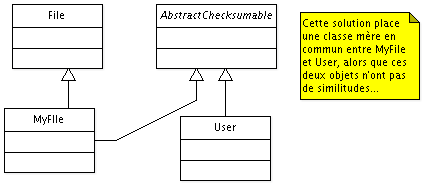
\includegraphics[bb=0 0 150 65]{../img/MultipleInheritance.png}
%  % MultipleInheritance.png: 150x65 pixel, 72dpi, 5.29x2.29 cm, bb=0 0 150 65
% \end{center}
\end{frame}

\begin{frame}
	\frametitle{Solutions à l'aide d'interface}
	\lstinputlisting{../examples/org/esme/samples/InterfaceUsage.java}
%	Néanmoins, quelle est la faiblesse de ce fonctionnement par rapport à l'héritage multiple ?
\end{frame}

\begin{frame}
	\frametitle{Limites par rapport à l'héritage multiple}
	\begin{block}{On n'hérite pas de l'implémentation !}
		\begin{itemize}
			\item Il faut coder 'checksum()' pour chaque classe !
			\item Cependant, en pratique, ce n'est pas un problème comme dans ce cas, car les implémentations requises pour une même méthode sur deux objets distincts sont généralement très différentes...
		\end{itemize}
	\end{block}	
	
	\begin{center}
		\textit{Pour s'en rendre compte, il suffit de réflechir à l'implémentation de checksum() 
		pour un fichier et pour un objet Utilisateur...}
	\end{center}
\end{frame}

\begin{frame}
	\begin{block}{Couplage lâche}
		\lstinputlisting{../examples/org/esme/samples/LooseCoupling.java}
	\end{block}
	\begin{center}
		En quoi cette solution est-elle \textit{meilleure} ?
	\end{center}
\end{frame}
\begin{frame}
	\begin{block}{Exemple d'utilisation}
		\lstinputlisting{../examples/org/esme/samples/LooseCouplingExample.java}
	\end{block}
\end{frame}

\subsection{Paquetage}
\begin{frame}

	\begin{block}{Pourquoi une notion de \textbf{package} ?}
		\begin{itemize}
			\item Pour assurer la séparation du code, sous forme de modules:
			\begin{itemize}
			\item \texttt{org.esme.tppoo.ihm}
			\item \texttt{org.esme.tppoo.process}
			\item \texttt{org.esme.tppoo.persistance}
			\end{itemize}		
		\item Pour assurer une \underline{unicité de type}
		\end{itemize}
	\end{block}

	\begin{block}{Convention de nommage}
		\begin{itemize}
			\item URL ``inversée'' (\texttt{org.esme.tppoo} par exemple)
			\item toujours en \textbf{minuscules},\textbf{pas de chiffres}
		\end{itemize}
	\end{block}
	\begin{block}{Convention pour les TPs}
	\texttt{org.esme.tppoo}, \texttt{org.esme.tpihm}, \texttt{org.esme.tpxml},...
	\end{block}
\end{frame}

\subsection{Collections}
\begin{frame}
	\begin{block}{Les Collections en Java}
	
		\begin{itemize}
			\item Tableaux d'objets, \textbf{alloués dynamiquement}
			\item Listes chainées ``génériques``:
			\begin{itemize}
				\item Simple (\texttt{Set})
				\item Ordonnées (\texttt{List})
				\item Indexées (\texttt{Map}) 
			\end{itemize}
			\item Elles peuvent aussi être triées (\texttt{SortedSet},\texttt{SortedMap})
			\item Depuis Java 5, elles sont \textbf{typées} ( \texttt{List\textbf{<String>}},...)
		\end{itemize}
	\end{block}
	\begin{block}{Utilisez les !}
	 	\begin{itemize}
	 		\item Plus simples d'utilisation
			\item Optimisées à chaque version de la machine virtuelle Java
	 	\end{itemize}
	\end{block}
\end{frame}
% \begin{frame}
% 	\begin{block}{Utilisation d'une List}
% 		\begin{center}
% 			\textbf{Qu'est ce qui \underline{peut ne pas} fonctionner comme prévu dans ce code ?}
% 		\end{center}
% 		\lstinputlisting{../examples/org/esme/samples/ListUsage.java}
% 	\end{block}
% \end{frame}

\begin{frame}
	\begin{block}{Utilisation d'une Map}
		\lstinputlisting{../examples/org/esme/samples/MapUsage.java}
	\end{block}
\end{frame}

\subsection{Exceptions}
\begin{frame}
	\frametitle{Gestion des exceptions}
	\begin{block}{Que faisiez vous en C pour gérer une erreur ?}
		\begin{itemize}
			\item Rien, le programme plante.
			\item Renvoyer pointeur NULL ou un code d'erreur (STATUS)
			\item Retourner une structure décrivant l'erreur : plus d'autre retour possible !
		\end{itemize}
	Java, comme C{\#} et même le C++, dispose d'un mécanisme d'\textbf{Exception} !
	\end{block}	
\end{frame}

\begin{frame}
	\begin{block}{Mécanisme}
		Quand on souhaite signaler une erreur à l'appelant, il suffit de ''jeter`` \textbf{(throws)} une exception décrivant l'erreur. Charge à l'appelant de ''l'attraper`` (catch), et d'agir en conséquences, ou de la ''jeter`` à son propre appelant...
	\end{block}
	\begin{center}
		\textbf{A votre avis, quels sont les avantages d'un tel mécanisme ?}
	\end{center}
\end{frame}

\begin{frame}
	\begin{block}{Avantages}
		\begin{itemize}
			\item La signature de la méthode est plus claire (les cas d'erreurs
				seront explicitement décrits)
			\item L'Exception contient toutes les informations pour analyser le problème.
			\item L'erreur est remontée à la couche appropriée
	% L'erreur pourra être gérée au ''bon`` niveau, et il n'est plus nécessaire de définir un mécanisme ''maison`` ( code de retour, structure,...) pour transmettre les informations relatives à l'exception.
		\end{itemize}
		\textit{Note: Toute exception hérite de la classe Exception ou Error, ou sinon elle implémente l'interface Throwable.}
	\end{block}
\end{frame}

\begin{frame}
	\lstinputlisting[first=3,last=4]{../examples/org/esme/samples/Developer.java}
\end{frame}

\begin{frame}
	\begin{block}{Utilisation des exceptions}
		\begin{itemize}
			\item Les exceptions sont souvent \textbf{peu ou mal utilisées} malgré leur rôle crucial.
			\item Java vient avec \textbf{5 exceptions déjà définies} pour les cas les plus courants :
				\begin{enumerate}
					\item \textbf{IllegalArgumentException} %: quand une valeur de paramètre est inappropriée ;
					\item \textbf{IllegalStateException} %: quand l'état de l'objet est inapproprié ;
					\item \textbf{IndexOutOfBoundsException} %: quand l'index du paramètre est hors limites ;
					\item \textbf{ConcurrentModificationException} %: quand une modification concurrente a été détectée ;
					\item \textbf{UnsupportedOperationException} %: quand l'objet ne supporte pas la méthode 
				\end{enumerate}
				\textit{Si aucune d'elle ne semble convenir à la situation, à vous de créer une exception adaptée au problème}.
			\item La conception des exceptions fait autant parti de la conception d'un programme en langage orienté objet que l'héritage !
		\end{itemize}
	\end{block}
\end{frame}

\section{Fonctionnalités Avancées}
% \subsection{Chargement de classe dynamique}
\begin{frame}
	\begin{block}{Fonctionnalités Avancées}
		\begin{itemize}
			\item Chargement dynamique de classe : \texttt{Classloading}
			\item API de \texttt{Reflexion}
		\end{itemize}
	\end{block}
\end{frame}

% \subsection{Réflexion}
% \begin{frame}
% 	TODO
% \end{frame}
\part{2}
\section{TD}
\subsection{{\'E}noncé}
\begin{frame}
	\begin{block}{Première partie}
		\begin{enumerate}
			\item  Réalisation de l'arborescence du projet ( src, docs, bin,...) : "A l'aide d'Eclipse, créer un nouveau projet Java ( New Project - \textgreater Java Project ). Quels répertoirs sont créés ? A quoi servent-ils ?".
			\item  Package : "Créer un nouveau paquetage dans le répertoire 'src' nommé  'org.esme.tppoo'."
			\item  Réalisation d'une classe d'exemple : "Créer une classe dans le paquetage org.esme.tppoo, nommée \textit{Version}. Cette classe disposera d'une méthode \textit{getVersion} qui renverra la chaîne \textbf{"1.0"}.
		\end{enumerate}
	\end{block}
\end{frame}
\begin{frame}
	\begin{block}{Deuxième partie}
		\begin{enumerate}
		\item  Réalisation d'un programme principal : "A l'aide d'Eclipse ( regardez les options du formulaire de création de classe ), créer un 'programme principal', où vous créerez une instance de votre objet Version et où vous utiliserez la méthode getVersion."
		\item  Utilisation du \textbf{Debugger}
			\begin{itemize}
				\item 	Fixer un point d'arrêt
				\item 	Examiner la valeur d'une variable
				\item	Changer la valeur d'une variable
			\end{itemize}
		\item Compilation et utilisation en ligne de commande ( en // à Eclipse) et avec Ant
		\end{enumerate}
	\end{block}
\end{frame}
% \begin{frame}
% 	\begin{itemize}
% 		\item  Utilisation du plugin PMD pour vérifier le code
% 		\item  TODO and FIXME tag.
% 	\end{itemize}
% \end{frame}
\end{document}
